% ОБЯЗАТЕЛЬНО ИМЕННО ТАКОЙ documentclass!
% (Основной кегль = 14pt, поэтому необходим extsizes)
% Формат, разумеется, А4
% article потому что стандарт не подразумевает разделов
% Глава = section, Параграф = subsection
% (понятия "глава" и "параграф" из стандарта)
\documentclass[a4paper,article,14pt]{extarticle}

% Подключаем главный пакет со всем необходимым
\usepackage{spbudiploma}

% Пакеты по желанию (самые распространенные)
% Хитрые мат. символы
\usepackage{euscript}
% Таблицы
\usepackage{longtable}
\usepackage{makecell}
% Картинки (можно встявлять даже pdf)
\usepackage[pdftex]{graphicx}

\usepackage{amsthm,amssymb, amsmath}
\usepackage{textcomp}


\begin{document}

% Титульник в файле titlepage.tex
% --------------------- Стандарт СПбГУ для ВКР --------------------------
% Автор: Тоскин Николай, itonik@me.com
% Если заметили ошибку, напишите на email
% Если хотите добавить изменение самостоятельно, GitHub: . PR-s welcome!
% Использованы материалы:
% habr.com/ru/post/144648/
% cpsconf.ru
% Текст:
% http://edu.spbu.ru/images/data/normativ_acts/local/20181030_10432_1.pdf
% Титульный лист:
% http://edu.spbu.ru/images/data/normativ_acts/local/20180703_6616_1.pdf
% -----------------------------------------------------------------------

% Титульный лист диплома СПбГУ
% Временное удаление foot на titlepage
\newgeometry{left=30mm, top=20mm, right=15mm, bottom=20mm, nohead, nofoot}
\begin{titlepage}
\begin{center}
% Первый символ съедается, первым знаком поставлен Ы
\text{Санкт--Петербургский государственный университет}\\
\textbf{Кафедра технологии программирования}

\vspace{22mm}

\textbf{\Large Бельков Роман Андреевич} \\[7mm]
% Название
\textbf{\large Научно-исследовательская практика}\\[12mm]
\textbf{\Large Калибровка рекомендательных систем. Поиск гетерогенного эффекта и нетипичных пользователей для задач рекомендаций контента}

\vspace{12mm}
Направление 01.03.02 \\«Прикладная математика и информатика»\\
Основная образовательная программа СВ.5005.2015
«Прикладная математика, фундаментальная информатика и программирование»\\

\vspace{18mm}

% Научный руководитель, рецензент
% Сходить в уч отдел и узнать, правильно ли
\begin{flushleft}
{\setlength{\leftskip}{23em}
 {Руководитель практики:} \\
 канд. техн. наук, \\
 доцент \\ Блеканов И. С. \\
}
\end{flushleft}

\vfill

{Санкт-Петербург}
\par{2020 г.}
\end{center}
\end{titlepage}
\restoregeometry
\addtocounter{page}{1}

% Содержание
\tableofcontents
\pagebreak


\specialsection{Введение}

В настоящее время, количество информации растет очень быстрыми 
темпами и чтобы предоставлять наиболее релевантную и полезную 
для пользователей информацию, 
в веб сервисах начали использовать рекомендательные системы.  
Рекомендательные системы обеспечивают персонализированный 
пользовательский опыт во многих различных областях применения, 
включая интернет-магазины, социальные сети и потоковое
воспроизведение музыки/видео.  
Рекомендательная система -- это алгоритм, который предсказывает
 наиболее интересные
 объекты для конкретного пользователя на основе некоторой 
 информации о нем.

 Одна из проблем, которые имеют рекомендательные системы -- это 
 удовлетворение не всех интересов пользователя, рассмотрим пример 
 рекомендательной системы фильмов.
 Если пользователь посмотрел, 80 артхаусных фильмов и 20 
 комедий, то вполне разумно ожидать, что персонализированный 
 список рекомендуемых фильмов будет состоять примерно из 80\% 
 артхаусных и 20\% комедий.  Калибровка -- это общая концепция машинного обучения, 
 и в последнее время она переживает возрождение в 
 контексте справедливости алгоритмов машинного обучения.
  
  
  Калибровка особенно важна в свете того факта,
   что рекомендательные системы, оптимизированные в сторону
    точности
  в обычном автономном режиме, могут легко привести к 
  рекомендациям, где меньшие интересы пользователя 
  вытесняются основными интересами пользователя.
 Со временем такие несбалансированные рекомендации несут 
 в себе риск постепенного сужения областей интересов 
 пользователя -- что аналогично эффекту пузыря фильтров.

\pagebreak


\specialsection{Постановка задачи}

Основная цель работы заключается в реализации алгоритма 
калибровки рекомендательных систем и сравнении с существующими решениями.
Реализуемый алгоритм должен не сильно ухудшать
точность работы рекомендательной системы, но в то же время 
учитывать все интересы пользователя.
\\

Для достижения цели были поставлены следующие задачи:
\begin{enumerate} 
    \item Обзор существующих методов калибровки рекомендательных систем.
    \item Реализация алгоритма на языке Python.
    \item Поиск или сбор данных и проверка реализованного метода на данных.
    \item Сравнение результатов с существующими методами.
  \end{enumerate}
  
\pagebreak

\specialsection{Обзор литературы}
Калибровка рекомендация на данный момент имеет несколько направлений,
 первое заключается в получении более справедливых рекомендаций, а второе 
 в учете всех интересов пользователя при генерации рекомендаций. 
 
 Рассмотрим первое направление. Как правило, в рекомендательных 
 системах речь идет о рекомендациях товаров пользователям. 
 Однако в контексте справедливости имеет смысл абстрагироваться
  от объектов и субъектов. Например, при рекомендациях предложений о 
  работе испытуемыми являются люди, которые могут подвергаться 
  дискриминации по признаку расы или пола; при поиске поездки 
  рекомендуемыми объектами являются таксисты; в социальных сетях 
  предложения друзей включают отдельных людей в качестве субъектов 
  и объектов. Таким образом, справедливость в рекомендателями 
  могут иметь несколько точек зрения, как описано в \cite{bib1}: 
  справедливость для субъектов, называются потребительской справедливостью или 
  C-справедливостью, а справедливость для объектов, называется 
  справедливостью производителя или P-справедливостью. 

  Дискриминация в рекомедательных системах является отдельной задачей,
  которая достаточно хорошо описана в статье об исследовании честности
  иснтрументов для прогнозирования рецидива преступлений \cite{bib2}. 

  Второе направление более сосредоточено на диверсификации, 
  полноте и разнообразии рекомендации. Основным интсрументом 
  калибровки является переранжирование списка уже сгенерированных
   рекомендаций. В работе \cite{bib3} используется выделение подпрофилей, 
   на основе положительных оценок, 
   для каждого пользователя, которые отражают 
   определенные интересы. Другой метод предлагают исследователи из 
   Netflix \cite{bib4}, он основан на расстоянии Кульбака-Лейблера, 
   которое применяется для опеределения схожести пользовательского 
   распределения и сгенерированнного. В исследовании \cite{bib5} 
   используется метод Сент-Лагю для выбора N наиболее релевантных и 
   разнообразных рекомендаций. Обычно метод Сент-Лагю применяется для 
   распределения мест в правительстве, но в рассмотренной работе, его 
   модифицировали для рекомендаций фильмов.
\pagebreak

\section{Обзор существующих решений в области калибровки рекомендательных систем}
\subsection{Обзор существующих сервисов и инструментов}
Рекомендательные системы все чаще используются в различных сервисах. 
Очень трудно найти сервис стримингового просмотра видео контента или 
прослушивания музыки, в котором бы не применялись рекомендательные 
механизмы. Рассмотрим крупнейшие сервисы, внедрившие рекомендательные
системы.

Наиболее часто рекомендации применяются для рекомендаций фильмов. 
\textbf{Netflix} -- одна из передовых компаний в области рекомендаций контента,
в которой на данный момент применятся огромное количество подходов и методов
для рекомендаций не только фильмов и сериалов, но и постеров, а иногда
для порядка серий. Но не одни Netflix занимаются видео контентом. 
\textbf{MovieLens} -- это веб-сайт, разработанный исследовательской группой
из университета Миннесоты GroupLens, который помогает людям найти фильмы
 для просмотра. У него есть сотни тысяч зарегистрированных 
 пользователей. В MovieLens проводят онлайн-полевые эксперименты в области автоматизированной рекомендации контента, 
  интерфейсов рекомендаций, основанных на тегировании рекомендателей
   и интерфейсов, баз данных, и 
   интеллектуального дизайна пользовательского интерфейса.

  Помимо фильмов довольно часто рекомендательные системы применяются
  в музыкальных сервисах, например \textbf{Last.FM} -- это веб-сайт, 
  который собирает данные о прослушивании пользователями композиций и
  с помощью алгоритма коллаборативной фильтрации,
  формирует персонализированный и общий хит-парад. 
  \textbf{Spotify} -- интернет сервис для потокового 
  прослушивания аудио. В этом сервисе применяется сразу несколько
  подходов в рекомендации композиций: первый, такой же как в Last.FM,
  основанный на поиске похожих пользователей, второй использует 
  обработку естественного языка для анализа тектов песен, третий
  построен на нейронной сети, которая обрабатывает аудио состовляющую композиций.

  Также, в последнее время, многи социальные сети начинают внедрять
  рекомендательные алгоритмы в свои сервисы. Так, например \textbf{Instagram}
  применяют собственный фреймворк ig2vec \cite{ig2vec}, основаный на 
  word2vec, для представления изображений в векторном виде, а дальше, 
  сравнивая вектора пользователей, в онлайн режиме формируют бесконечную
  персонализированную ленту изображений.

  Из открытых инструментов для построения рекомендательных систем, мне
  удалось найти фреймворк \textbf{SurPRISE} \cite{sur} для языка программирования Python, 
  реализованный с помощью SciKits \cite{SciKits} (сокращенно от scipy Toolkits) -- 
  это дополнительные пакеты для SciPy \cite{Scipy}, размещенные и разработанные 
  отдельно и независимо от основного дистрибутива SciPy. SciPy -- 
  это основанная на Python экосистема программного обеспечения с 
  открытым исходным кодом для математики, естественных наук и 
  инженерии.

\subsection{Обзор методов калибровки рекомедательных систем}
\subsubsection{Расстояние Кульбака-Лейблера}
В ходе работы был проведен обзор литературы и найдено два 
метода потенциально подходящих для решения поставленной проблемы. 
Первый метод заключается в пересчете целевой метрики с помощью 
расстояния Кульбака-Лейблера (\ref{eq:KL}) \cite{bib4}.
\begin{equation}
  C_{KL}(p,q) = KL(p||\tilde{q}) = \sum_g p(g|u)\log\frac{p(g|u)}{\tilde{q}(q|u)},
  \label{eq:KL}
\end{equation}
где ${p}$ это целевое распределение жанра ${g}$ для пользователя 
$u$, $q$ -- полученное распределение жанров для пользователя.
Во избежание случая $q(g|u)=0$, будем использовать 
\begin{equation}
  \tilde{q}(q|u) = (1-\alpha) \cdot q(g|u) + \alpha \cdot p(g|u)
\end{equation} с очень маленьким $\alpha>0$, такое что $q\approx\tilde{q}$.

Сама же калибровка выполняется по формуле: 
\begin{equation}
  \label{eq:Calibrated}
  I^*=\arg \max_{I, |I|=N} (1-\lambda) \cdot s(I) - \lambda \cdot C_{KL}(p,q(I)),
\end{equation} где $\lambda \in [0,1]$, которая определяет 
компромисс между расстоянием Кульбака-Лейблера и значением 
метрики полученным рекомендательной системой. $s(I)=\sum_{i\in I}s(i)$, 
где $s(i)$ -- степень уверенности, что фильм $i$ подойдет 
пользователю, предсказанная рекомендательной системой.
\subsubsection{Метод Сент-Лагю}
Второй алгоритм является адаптацией метода Сент-Лагю. \cite{bib5} 
Метод Сент-Лагю, был изобретен французским математиком Андре 
Сент-Лагю для пропорционального распределения мандатов в 
правительстве. Суть метода заключается в поочередном присуждении 
мандатов партии с наибольшей квотой, которая на кажом шаге 
считается по формуле $\frac{V}{2s+1}$, где $V$ -- количество 
голосов, полученных партией, s -- количество мандатов, 
выделенных партии на данном шаге.

Можно модифицировать данный метод под наш случай. 
Имея список наиболее релевантных фильмов, мы будем 
формировать новый список, выбирая фильмы по одному 
методом Сент-Лагю, только вместо партий у нас будут 
жанры, а голоса, полученные партией, заменятся на количество 
понравившихся пользователю фильмов конкретного жанра.

\subsection{Обзор метрик качества методов калибровки рекомендаций}
В качестве метрики качества рекомендательной системы будет 
использоваться точность (\ref{eq:prec}) (precission) --  это доля релевантных экземпляров 
среди извлеченных экземпляров \cite{bib6}, также называемая положительная 
прогностическая ценность и расчитывается по формуле \begin{equation}
    Precision = \frac{tp}{tp+tn},
    \label{eq:prec}
  \end{equation}
  где ${tp}$ -- true positive, количество элементов корректно принятых алгоритмом, 
  ${tn}$ -- true negative, количество элементов корректно отклоненных алгоримтом. 
  В нашем случае ${tp}$ будет количеством элементов, которые рекомендательная система 
  порекомендует верно, а ${tn}$ -- количество элементов верно не рекомендованных алгоритмом.

Если же рекомендательная система работает не как бинарный классификатор, рекомендовать
определенный элемент пользователю или нет, но и предсказывает, например оценку этого
элемента конкретным пользователем, то можно использовать две похожие между собой метрики
MSE (\ref{eq:mse}) (mean squared error) -- среднеквадратичная ошибка и RSME (\ref{eq:rmse}) 
(root mean squared error) -- корень среднеквадратичной ошибки.
\begin{equation}
    MSE = \frac{1}{n}\sum_{i=1}^n(Y_i-\hat Y_i)^2,
    \label{eq:mse}
  \end{equation}
  где ${n}$ -- это количество предсказаний,  ${Y_i}$ реальные значения 
  предсказываемой величины, ${\hat Y_i}$ предсказанные значения.
  \begin{equation}
    RMSE = \sqrt{\frac{1}{n}\sum_{i=1}^n(Y_i-\hat Y_i)^2}.
    \label{eq:rmse}
  \end{equation}

  Для вычисления схожести распределения реальных интересов пользователя и распределеня, 
  полученного рекомендательной системой, имеется несколько метрик. Первый способ, это
  использование критерия согласия Пирсона \cite{bib7}, это непараметрический критерий,
  который применяют для проверки гипотезы о соответствии эмпирического распределения предполагаемому.
  Статистика критерия Пирсона вычисляется по формуле (\ref{eq:Pirson})
  \begin{equation}
    \chi^2 = \sum_{i=1}^n\frac{(k_i-p_i)^2}{p_i},
    \label{eq:Pirson}
  \end{equation}
  где ${n}$ -- количество
  классов в распределении величины, ${k_i}$ -- фактические частоты встречаемости величины в ${i}$-ом классе,
  ${p_i}$ -- ожидаемые частоты встречаемости величины в ${i}$-ом классе. Чем меньше эта статистика, тем более схожи между собой распределения.

  Еще один метод оценки схожести распределений предложен в статье от Netflix \cite{bib4}, 
  там используется дивергенция Кульбака-Лейблера (\ref{eq:KL}) из класса ${f}$-дивергенций ${\displaystyle D_{f}(P\parallel Q)}$,  определяющих в общем случае несимметричную меру расхождения между двумя распределениями вероятностей ${P}$ и ${Q}$.


\pagebreak

\section{Реализация программного комплекса калибровки результатов рекомендательных системы}
\subsection{Выбор технологий и инструментов для реализации}
Для программной реализации методов калибровки рекомендательных систем были выбраны следующие инструменты:
\begin{itemize} 
    \item Python3 -- скриптовый динамический язык программирования, 
    выбран для реализации методов и использования готовых библиотек.
    \item SurPrise \cite{sur} -- фреймворк для языка программирования Python
    с готовой реализацией нескольких методов рекомендательных систем.
    \item SciPy \cite{Scipy} -- это бесплатная библиотека Python с открытым исходным кодом, используемая для научных вычислений и технических вычислений.
    \item Implicit \cite{imp} -- библиотека с реализованной коллаборативной фильтрацией для неизвестных данных.
  \end{itemize}

\subsection{Алгоритм рекомендательной системы}

В качестве алгоритма рекомендаций было выбрано Байесовское 
персонализированное ранжирование \cite{bib8}. 
Основная задача персонализированного ранжирования состоит 
в том, чтобы предоставить пользователю ранжированный список 
элементов.

Пусть ${U}$-множество всех пользователей,а ${I}$-множество всех 
элементов. Ниже на рисунке \ref{BPR1} показано, как обрабатываются неявные 
данные в случае общих рекомендателей элементов.
\begin{figure}[ht]
    \begin{center}
    \scalebox{0.35}{
       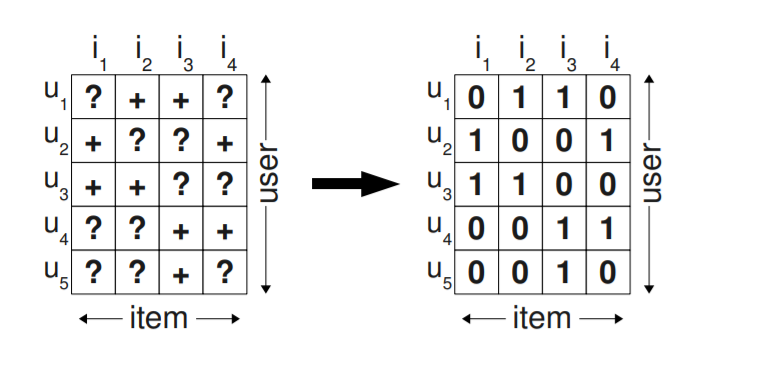
\includegraphics{images/BPR1.png}
    }
    
    \caption{
    \label{BPR1}
         }
    \end {center}
    \end {figure}
    Обычный подход заключается в том, чтобы предсказать
     персонализированную оценку для элемента, которая отражает 
     предпочтения пользователя для этого элемента. После этого 
     предметы будут ранжированы на основе этого балла. Здесь,
      как вы можете видеть на рисунке \ref{BPR1}, все существующие 
      взаимодействия между Пользователем и элементом помечаются как 
      положительный класс(1), а остальные взаимодействия помечаются
      как отрицательный класс(0).

      В подходе Байесовского
      персонализированного ранжирования, вместо взятия одного элемента, 
      будут рассматриваться пары элементов как обучающие данные.  Набор
         данных, который будет рассматриваться, сформулирован следующим
          образом 
          \begin{equation}
            (u,i,j) \in D_S
            \label{eq:1}
          \end{equation}
          
          \begin{figure}[ht]
            \begin{center}
            \scalebox{0.3}{
               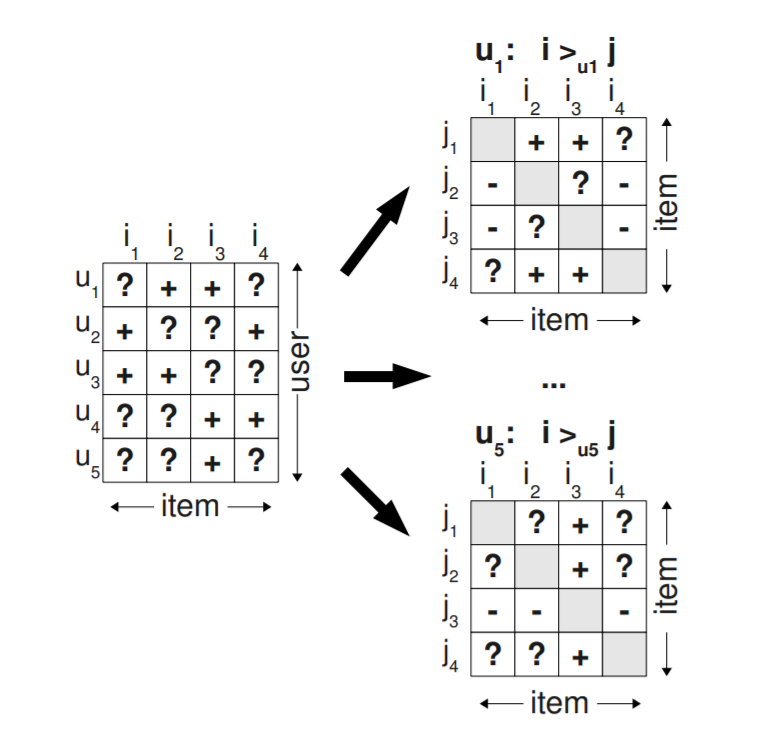
\includegraphics{images/BPR2.png}
            }
            
            \caption{
            \label{BPR2}
                 }
            \end {center}
            \end {figure}

            Здесь триплеты, сгенерированные для обучающих данных, представляют собой специфические для пользователя попарные предпочтения между парой элементов.
            

      \begin{equation}
        p(\Theta| >_u) \propto p(>_u| \Theta)p(\Theta)
        \label{eq:lik}
      \end{equation}

      Функция правдоподобия (\ref{eq:lik}), где ${>_u}$ -- это необходимые, 
      но латентные предпочтения структуры для пользователя $u$.

      Предполагая, что пользователи будут действовать независимо и порядок 
      каждой пары элементов ${(i, j)}$ для конкретного пользователя не зависит 
      от порядка каждой другой пары, мы можем сформулировать индивидуальную 
      вероятность того, что пользователь предпочитает элемент $i$ элементу $j$ 
      следующим образом:
      \begin{equation}
        p(i >_u j|\Theta) := \sigma(\hat x_{uij}(\Theta))
        \label{eq:ver}
      \end{equation}
    где $\sigma$ логистическая сигмоида: 
    \begin{equation}
        \sigma(x) := \frac{1}{1+e^{-x}}
        \label{eq:sigm}
      \end{equation}

${\hat x_{uij}(\Theta)}$ -- это в приведенном выше уравнении (\ref{eq:ver}) является 
вещественной значимой функцией, которая представляет собой отношение 
между пользователем $u$, элементом $i$ и элементом $j$ и обычно вычисляется 
с использованием модели матричного факторизации. Сигмовидная 
функция (\ref{eq:sigm}) дает индивидуальную вероятность, которая будет оптимизирована в 
ходе процесса.

${p(\Theta)}$ - это априорная вероятность, представляющая собой нормальное 
распределение с нулевым средним и дисперсионно-ковариационной матрицей.
\begin{equation}
    p(\Theta) \sim N(0, \Sigma_{\Theta})
    \label{eq:apr}
  \end{equation} 

  Следующее уравнение (\ref{eq:opt}) является окончательным критерием Байесовского
  персонализированного ранжирования, который должен быть оптимизирован
  \begin{equation}
    \sum_{(u,i,j)\in D_S} \ln \sigma(\hat x_{uij}) - \lambda_\Theta||\Theta||^2
    \label{eq:opt}
  \end{equation} 
  где $\lambda_\Theta$ -- специфические параметры регуляризации модели.

  \subsection{Реализация на языке программирования Python}
  Выберем порог оценки элемента, выше которого оценка считается положительной.
  Для дальнейшей работы представляем данные в виде разряженной таблицы, для более быстрой работы с большими таблицами.
  Разделяем исходные данные на тренировочную и тестовую выборки, 80\% данных на 
  тренировочную и 20\% на тестовую. На тренировочной выборке строим алгоритм рекомендаций байесовского
  персонализированного ранжирования.

  Далее реализуем метрики для проверки качества полученных рекомендаций.
  В качестве метрики для проверки точности рекомендаций используем precision (\ref{eq:prec}) (точность),
  а в качестве метрики сравнения исходного распределения и полученного, будем использовать
  дивергенцию Кульбака-Лейблера (\ref{eq:KL}). Для проверки будем брать
  30 лучших рекомндаций для пользователя.

  Калибровку рекомедаций будем производить двумя методами: первый (\ref{eq:Calibrated})
  основан на дивергенции Кульбака-Лейблера, а второй является 
  адаптацией метода Сент-Лагю \cite{bib5}.

Для сравнения с готовым решением будем использовать фреймворк SurPRISE \cite{sur} на языке программирования Python.
Из набора реализованных во фреймворке методов используем основанный на предположении о нормальном распределении NormalPredictor.

\pagebreak

\section{Проведение эксперимента}
\subsection{Постановка эксперимента}
Для проверки качества и сравнения алгоритмов было поставлено 3 эксперимента:
\begin{itemize}
   \item Построение рекомендаций Байесовским
   персонализированным ранжированием и калибровка методом Кульбака-Лейблера \cite{bib4}.
   \item Построение рекомендаций Байесовским
   персонализированным ранжированием и калибровка методом Сент-Лагю \cite{bib5}.
   \item Построение рекомендаций с помощью готового фреймворка SurPRISE \cite{sur}.
\end{itemize}
\subsection{Набор данных}
Для проведения эксперимента был выбран датасет MovieLens 25M \cite{voc3}, включающий в себя 25 миллионов оценок к 62,000 фильмов от 162,000 пользователей.
Данные представленны в виде двух csv файлах. Первый rating.csv состоит из
четырех колонок: userId -- id пользователя, moviesId -- id фильма, 
rating -- оценка, поставленная по пятибальной шкале, пользователем для данного фильма,
timestamp -- временная отметка оценки.
   \begin{center}
   \begin{tabular}{ | r  | l | l | l |}
      \hline
      userId & movieId & rating & timestamp  \\ \hline
      1 & 2 & 3.5 & 1112486027 \\
      1 & 29 & 3.5 & 1112486676 \\
      1 & 32 & 3.5 & 1112486819\\
      1 & 47 & 3.5 & 1112486727 \\
      1 & 50 & 3.5 & 1112486580 \\
      1 & 112 & 3.5 & 1112486740 \\
      1 & 151 & 4 & 1112486734 \\
      1 & 223 & 4 & 1112486573 \\
      1 & 253 & 4 & 1112486940 \\
      1 & 260 & 4 & 1112486826 \\
      \hline
      \end{tabular}
   \end{center}
Второй файл movies.csv состоит из трех столбцов: moviesId -- id фильма, 
title -- название фильма, genres -- жанры, к которым относится фильм.
   \begin{center}
      \scalebox{0.9}{
      \begin{tabular}{ | r | l | l |}
         \hline
         movieId & title & genres \\ \hline
         1 & Toy Story (1995) & Adventure|Animation|Children|Comedy|Fantasy \\
         2 & Jumanji (1995) & Adventure|Children|Fantasy \\
         3 & Grumpier Old Men (1995) & Comedy|Romance \\
         4 & Waiting to Exhale (1995) & Comedy|Drama|Romance \\
         5 & Father of the Bride Part II (1995) & Comedy \\
         6 & Heat (1995) & Action|Crime|Thriller \\
         7 & Sabrina (1995) & Comedy|Romance \\
         8 & Tom and Huck (1995) & Adventure|Children \\
         9 & Sudden Death (1995) & Action \\
         10 & GoldenEye (1995) & Action|Adventure|Thriller \\
         \hline
         \end{tabular}
      }
      \end{center}

Во фреймворке SurPRISE \cite{sur} встроены несколько наборов данных, например MovieLens 1M, но для 
более честного сравнения, будем вручную загружать набор MovieLens 25M.
\subsection{Результаты}

В результате эксперимента 1 была произведена калибровка рекомендаций и подбор коэффициента $\lambda$ для калибровки Кульбака-Лейблера (\ref{eq:Calibrated})
и были получены следующие результаты:
\begin{center}
   \scalebox{1}{
   \begin{tabular}{ | r | c | l |}
      \hline
      $\lambda$ & Precision & $C_{KL}$ \\ \hline
      ${\lambda =0}$ (нет калибровки) & 0.43 & 0.93 \\
      ${\lambda =0.2}$ & 0.49 & 0.47 \\
      ${\lambda =0.3}$ & 0.45 & 0.39 \\
      ${\lambda =0.5}$ & 0.33 & 0.31 \\
      ${\lambda =0.7}$ & 0.21 & 0.25 \\
      ${\lambda =0.8}$ & 0.18 & 0.11 \\
      ${\lambda =0.99}$ & 0.14 & 0.019 \\
      \hline
      \end{tabular}
   }
   \end{center}
Заметно, что с увеличением $\lambda$ идет уменьшение дивергенции Кульбака-Лейблера между распределениями, следовательно
полученные рекомендации больше поможи на интересы пользователя. Но также 
с увеличением $\lambda$ идет сначала небольшой рост точности, а после ее снижение.
Для наилучшего результата, я считаю оптимальным взять $\lambda=0.3$.

В эксперименте 2 после применения калибровки адаптированным методом Сент-Лагю \cite{bib5}, получились следующие результаты:
\begin{center}
   \scalebox{1}{
   \begin{tabular}{ | r | l |}
      \hline
      Precision & $C_{KL}$ \\ \hline
         0.12 & 0.3 \\
      \hline
      \end{tabular}
   }
   \end{center}
Точность получилась заметно хуже исходной, а сходство полученного
распределения интересов пользователя с реальным заметно меньше, чем 
при калибровке Кульбака-Лейблера с таким же показателем точности.

Эксперимент 3, при использовании готового фреймворка, показал достаточно хорошие результаты:
\begin{center}
   \scalebox{1}{
   \begin{tabular}{ | r | l |}
      \hline
      Precision & $C_{KL}$ \\ \hline
         0.53 & 0.61 \\
      \hline
      \end{tabular}
   }
   \end{center}
этот метод показывает наилучшую точность, но не впечатляющие значения дивергенции Кульбака-Лейблера.

Для более наглядной демонстрации результатов привожу несколько графиков для сравнения распределений интересов пользователя.
На графике отобразим долю каждого жанра среди интересов для пользователей. 
Синим цветом обонзачены исходные данные, на которых обучались алгоримы,
оранжевым цветом обозначены данные, полученные рекомендательной системой,
а зеленым цветом обонзачены откалиброванные данные, сгенерированные рекомендательной системой.
\begin{figure}[ht]
   \begin{flushleft}
      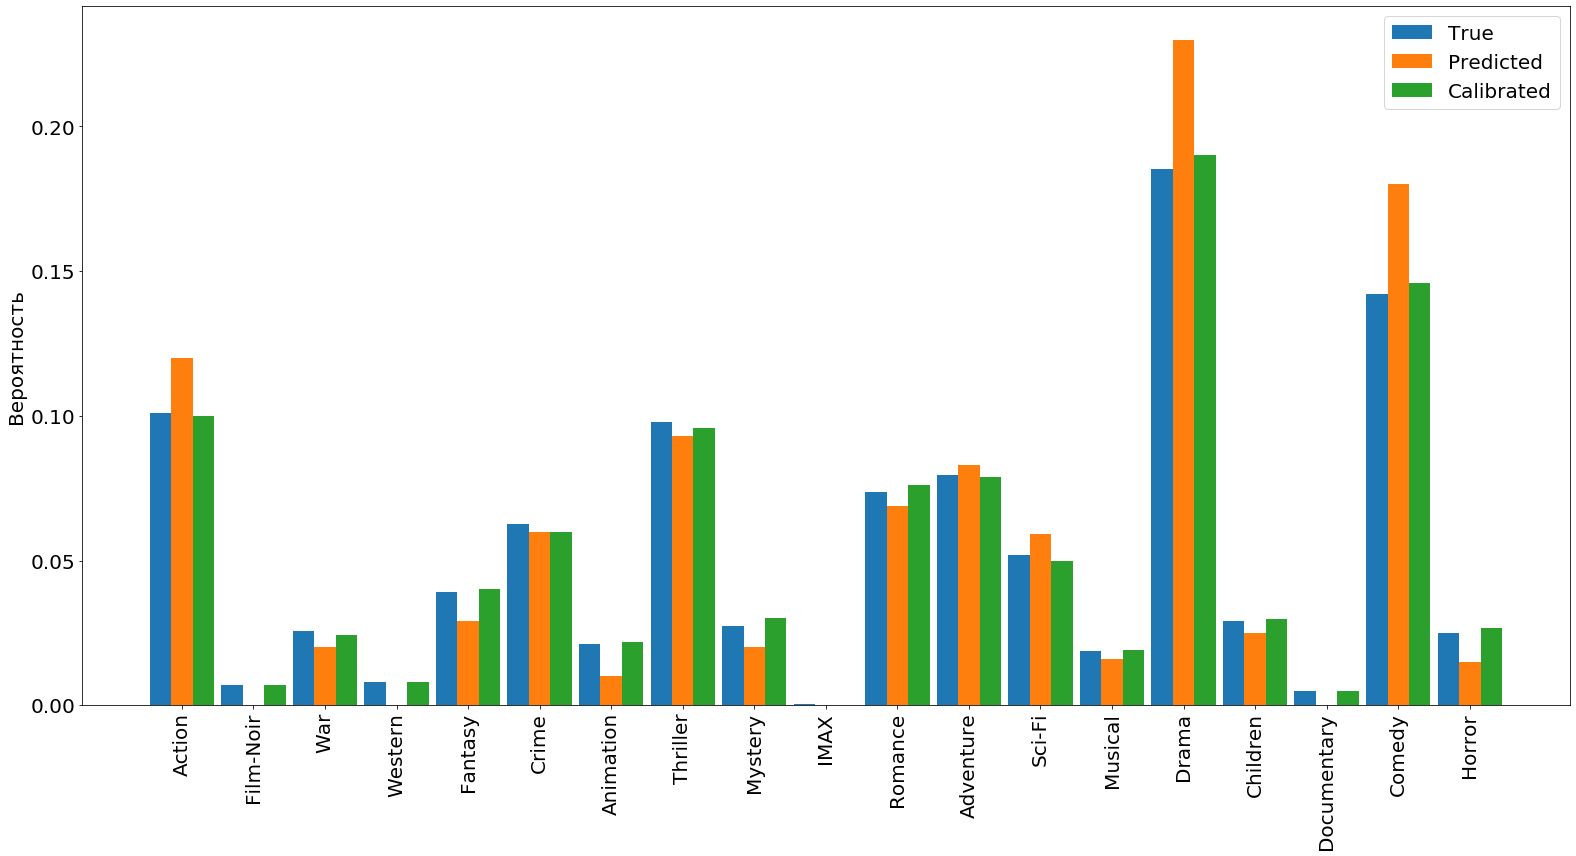
\includegraphics[width=17.5cm, height=10cm]{images/bay.png}
   
   \caption{
   \label{graph-KL}
        Распределение жанров при Байесовском персонализированном ранжировании.}
   \end {flushleft}

   \end {figure}

\pagebreak

На рисунке \ref{graph-KL} демнострируется эффект калибровки Кульбака-Лейблера с ${\lambda=0.3}$ для Байесовского персонализированного ранжирования.
Заметно, что жанры, которые больше остальных представлены в обучающих данных, выдаются рекомендательной системой еще чаще,
в то время как калибровка приближает данные к реальным. С малочисленными жанрами ситуация обстоит немного иначе,
Байесовское персонализированное ранжирование не представило некоторые жанры, например вестерн и документальное кино, калибровка же
исправила это упущение. Таким образом, можно сделать вывод, что калиброванные рекомендации
намного лучше удовлетворяют интересы пользователя.


\pagebreak

   \begin{figure}[ht]
   \begin{flushleft}
      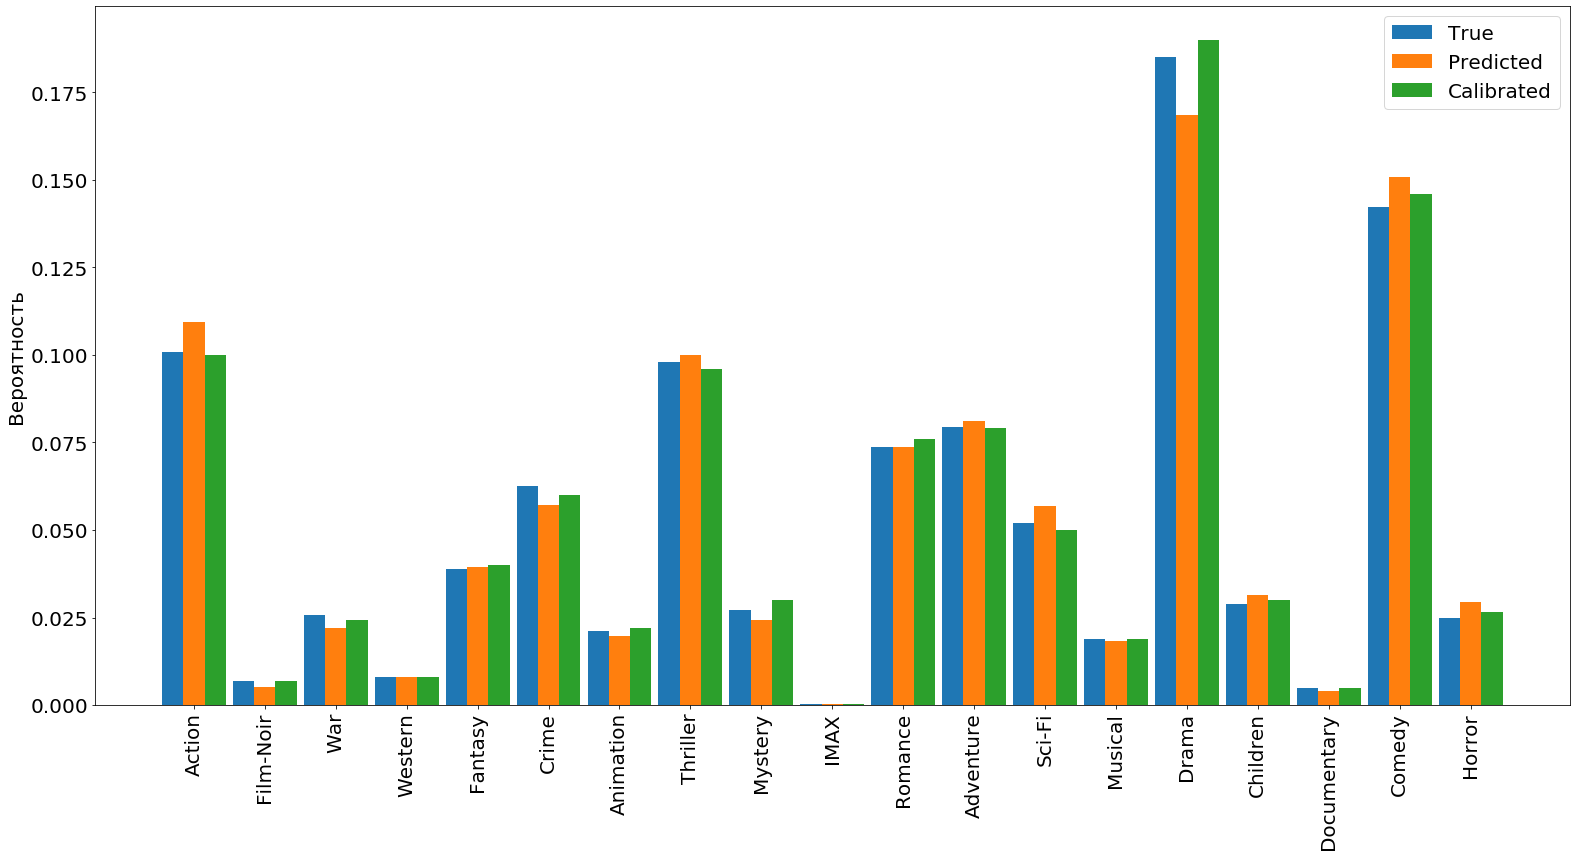
\includegraphics[width=17.5cm, height=10cm]{images/cal_surp.png}
   
   \caption{
   \label{graph-SUR}
        Распределение жанров при использовании фреймворка SurPRISE.}
   \end {flushleft}
   \end {figure}



      На рисунке \ref{graph-SUR} сравниваются распределения, фареймворком SurPRISE и калибровкой Кульбака-Лейблера с ${\lambda=0.3}$ для Байесовского персонализированного ранжирования.
      Тут уже нет серьезных проблем со стороны рекомендательной системы, все жанры представлены и
      имеют долю достаточно близкую к реальной. Калибровка в этом случае показывает все еще лучший результат, но разница уже не так велика.

      По итогам экспериментов, можно сказать, что калибровка показала отличные результаты,
      интересы ползователей удовлетворяются достаточно хорошо и распределение жанров получается близким к реальному.
      Точность при калибровке может немного снизится, но я считаю, что пользовательский опыт при этом не пострадает, так как их интересы будут более широко представлены.


\pagebreak


\pagebreak

\specialsection{Заключение}
\subsection*{Итоги работы}
В рамках работы были выполнены следующие задачи:
\begin{itemize}
    \item Обзор литературы на тему рекомендательных систем и их калибровки;
    \item Обзор существующих методов решения проблемы;
    \item Изучены и реализованы, на языке Python, два алгоритма калибровки рекомендаций;
    \item Проведены эксперименты на выбранном наборе данных;
    \item Проведено сравнение полученных результатов калибровки между собой и с готовой реализацией из фреймворка;
    \item Построены графики для наглядного сравнения распределения классов интересов пользователей.
\end{itemize}

Цель работы была достигнута, реализованный алгоритм калибровки рекомендательных систем
заметно улучшает учет пользовательских интересов в рекомндациях и немного повышает точность рекомендаций.
В сравнении с готовым решением, калибровка все еще лучше в плане удовлетворения пользовательских интересов, 
но по точности немного проигрывает.

\subsection*{Практическое применение}
Реализованный алгорит можно применять практически в любой рекомендательной системе, где фигурируют какие-то классы объктов рекомендаций, а не только для фильмов, как представлено в эксперименте.
Например в музыкальных сервисах можно заменить жанры фильмов на жанры музыки и использовать тот же метод.
В социальных сетях вместо жанров можно использовать теги записей, направленность группп и каналов. В новостных агрегаторах ориентироваться на тематику новости.
В интернет-магазинах классами будут являться категории товаров.

\subsection*{Дальнейшее развитие}
В дальнейшем для улучшение алгоритма, можно заменить метод применяемы рекомендательной системой на более точный и калибровать его результаты,
возможно точность в этом случает будет даже выше, чем в готовом фреймворке. Также, можно попробовать реализовать идею применения нескольких методов калибровки последовательно.


\pagebreak

% Библиография в cpsconf стиле
% Аргумент {1} ниже включает переопределенный стиль с выравниванием слева
\begin{thebibliography}{1}
\bibitem{bib1} Robin Burke \flqq Multisided Fairness for Recommendation\frqq. Presented as a poster at the 2017 Workshop on Fairness, Accountability, and Transparency in Machine Learning (FAT/ML 2017), \href{https://arxiv.org/pdf/1707.00093.pdf}{arxiv.org/pdf/1707.00093.pdf}.
\bibitem{bib2} Alexandra Chouldechova \flqq Fair prediction with disparate impact: A study of bias in recidivism prediction instruments\frqq. FATML 2016 conference paper. A long version of the paper available on the author's website, \href{https://arxiv.org/pdf/1610.07524.pdf}{arxiv.org/pdf/1610.07524.pdf}.
\bibitem{bib3} Mesut Kaya, Derek Bridge \flqq Accurate and Diverse Recommendations Using Item-Based SubProfiles\frqq. 	hirty-First International Florida Artificial Intelligence Research Society Conference, 2018, pp. 462--467 \href{https://www.insight-centre.org/sites/default/files/publications/kaya-bridge-2017.pdf}{www.insight-centre.org/sites/default/files/publications/kaya-bridge-2017.pdf}.
\bibitem{bib4} Harald Steck \flqq Calibrated Recommendations\frqq. RecSys '18: Proceedings of the 12th ACM Conference on Recommender Systems, 2018, pp. 154--162, \href{https://doi.org/10.1145/3240323.3240372}{doi.org/10.1145/3240323.3240372}.
\bibitem{bib5} Van Dang and W. Bruce Croft \flqq Diversity by Proportionality: An Election-based Approach to Search Result Diversification\frqq. SIGIR '12: Proceedings of the 35th international ACM SIGIR conference on Research and development in information retrieval, 2012, pp. 65--74, \href{https://doi.org/10.1145/2348283.2348296}{doi.org/10.1145/2348283.2348296}.
\bibitem{bib6} David M W Powers \flqq Evaluation: From Precision, Recall and F-Factor to ROC, Informedness, Markedness and Correlation\frqq. Journal of Machine Learning Technologies, 2011, pp. 37--63, \href{https://csem.flinders.edu.au/research/techreps/SIE07001.pdf}{csem.flinders.edu.au/research/techreps/SIE07001.pdf}.
\bibitem{bib7} Кендалл М., Стьюарт А. \flqq Статистические выводы и связи\frqq. Наука, 1973.
\bibitem{ig2vec} Ivan Medvedev, Haotian Wu, Taylor Gordon \flqq Powered by AI: Instagram’s Explore recommender system\frqq. Facebook Artificial Intelligence, 2019.
\bibitem{sur} Nicolas Hug \flqq Surprise a Python library for recommender systems\frqq, 2017. \href{http://surpriselib.com}{surpriselib.com}.
\bibitem{SciKits} Официальный сайт документации SciKits: \href{https://www.scipy.org/scikits.html}{www.scipy.org/scikits.html}.
\bibitem{Scipy} Pauli Virtanen, Ralf Gommers, Travis E. Oliphant,
Matt Haberland, Tyler Reddy, David Cournapeau, Evgeni Burovski,
Pearu Peterson, Warren Weckesser, Jonathan Bright, St{\'e}fan J. van der Walt,
Matthew Brett, Joshua Wilson,  Jarrod K. Millman, Nikolay Mayorov, 
Andrew Nelson, Eric Jones, Robert Kern,  Eric Larson,
CJ Carey, {\.I}lhan Polat,  Yu {Feng},  Eric W. {Moore},
Jake {Vand erPlas},  Denis {Laxalde},  Josef
{Perktold},  Robert {Cimrman},  Ian {Henriksen},  E.~A.
{Quintero},  Charles R {Harris},  Anne M. {Archibald}, 
Ant{\^o}nio H. {Ribeiro},  Fabian {Pedregosa},  Paul
{van Mulbregt} \flqq SciPy 1.0: Fundamental Algorithms for Scientific
Computing in Python\frqq. Nature Methods 2020, \href{https://doi.org/10.1038/s41592-019-0686-2}{doi.org/10.1038/s41592-019-0686-2}.
\bibitem{pandas} The pandas development team \flqq pandas: powerful Python data analysis toolkit\frqq. \href{https://pandas.pydata.org/docs/pandas.pdf}{pandas.pydata.org/docs/pandas.pdf}.
\bibitem{numpy} Travis E. Oliphant. \flqq A guide to NumPy\frqq. USA: Trelgol Publishing, 2006. \href{https://numpy.org/doc/stable/}{numpy.org/doc/stable}.
\bibitem{plot} Hunter, J. D. \flqq Matplotlib: A 2D graphics environment\frqq. Computing in Science \& Engineering vol. 9, no. 3, pp. 90-95, 2007. \href{https://matplotlib.org/citing.html}{matplotlib.org/citing.html}.
\bibitem{imp} Официальный сайт документации Implicit: \href{https://implicit.readthedocs.io/en/latest/quickstart.html}{implicit.readthedocs.io/en/latest/quickstart.html}.
\bibitem{bib8} Steffen Rendle, Christoph Freudenthaler, Zeno Gantner, Lars Schmidt-Thieme \flqq BPR: Bayesian Personalized Ranking from Implicit Feedback\frqq. 	Appears in Proceedings of the Twenty-Fifth Conference on Uncertainty in Artificial Intelligence (UAI2009), \href{https://arxiv.org/abs/1205.2618}{arxiv.org/abs/1205.2618}.
\bibitem{voc3} F. Maxwell Harper and Joseph A. Konstan \flqq ACM Transactions on Interactive Intelligent Systems\frqq. ACM Trans. Interact. Intell. Syst. 5, 4, Article 19, 2015, \href{https://doi.org/10.1145/2827872}{doi.org/10.1145/2827872}.
\end{thebibliography}
\end{document}